\documentclass[tikz, border=6pt]{standalone}
\IfFileExists{lmodern.sty}{\usepackage[T1]{fontenc}\usepackage{lmodern}}{}
\usepackage{amsmath,amssymb,bm}
\usetikzlibrary{arrows.meta, automata}
\definecolor{Blue}{HTML}{3A76D8}
\definecolor{Ink}{HTML}{1F2937}
\tikzset{
  state node/.style={/utils/exec={\colorlet{pytikzarg}{#1}}, state, draw=pytikzarg!78!black, fill=pytikzarg!20, minimum size=9.5mm, inner sep=1pt, line width=0.7pt, font=\small},
  state node/.default=Blue,
  transition/.style={Ink!80, line width=0.8pt, ->, shorten >=1pt},
  transition label/.style={font=\small, auto, inner sep=2pt},
}
\begin{document}
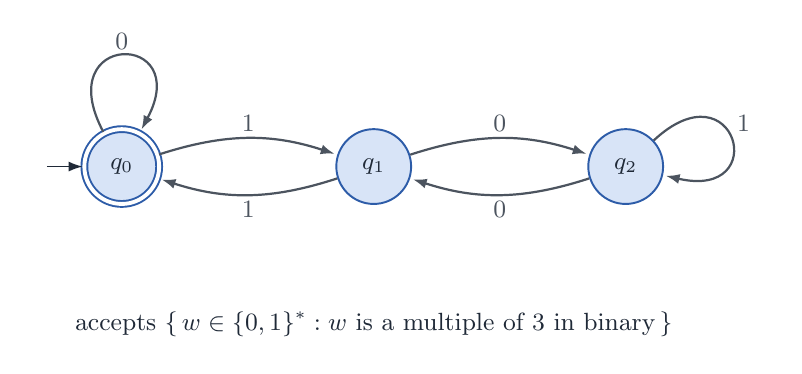
\begin{tikzpicture}[color=Ink, line width=0.5pt, >={Latex[length=5pt, width=3.6pt]}, line join=round]
  % graph fsm: 3 nodes, 6 edges
  \node[state node=Blue, initial, initial where=left, initial text=, accepting, double distance=1.4pt] (fsm-q-0) at (0,0) {$q_0$};
  \node[state node=Blue] (fsm-q-1) at (3.2,0) {$q_1$};
  \node[state node=Blue] (fsm-q-2) at (6.4,0) {$q_2$};
  \draw[transition] (fsm-q-0) to[out=118, in=62, looseness=8, min distance=5mm] node[transition label] {$0$} (fsm-q-0);
  \draw[transition] (fsm-q-0) to[bend left=18] node[transition label] {$1$} (fsm-q-1);
  \draw[transition] (fsm-q-1) to[bend left=18] node[transition label] {$0$} (fsm-q-2);
  \draw[transition] (fsm-q-1) to[bend left=18] node[transition label] {$1$} (fsm-q-0);
  \draw[transition] (fsm-q-2) to[bend left=18] node[transition label] {$0$} (fsm-q-1);
  \draw[transition] (fsm-q-2) to[out=43, in=-13, looseness=8, min distance=5mm] node[transition label] {$1$} (fsm-q-2);
  \node[font=\small] at (3.2,-2) {accepts $\{\,w \in \{0,1\}^* : w \text{ is a multiple of } 3 \text{ in binary}\,\}$};
\end{tikzpicture}
\end{document}
